\chapter{Proposal}
\label{chapter:proposal}

In this chapter we will define concepts that will be necessary to fully understand our proposal, which was developed in order to achieve the objectives presented in section \ref{sec:objectives}. In the last section we will expand on the criteria for what makes a good video-game map.

\section{Video-game maps}

In the context of video games, a map corresponds to a game scenery inhabited by the player and other entities like monsters, NPCs, objects, etc \cite{carvalho:2011}. The specific type of map that we have selected for this work is the 2D top-down type. This map perspective, also sometimes referred to as overhead view, bird's-eye view, Godview, etc. have a camera angle that shows the player and the area around them from above. An example of a game with an overhead view is shown in Figure \ref{fig:pokemon}.

\begin{figure}[h]
    \caption{Screenshot of Pokémon Gold gameplay}
    \centerline{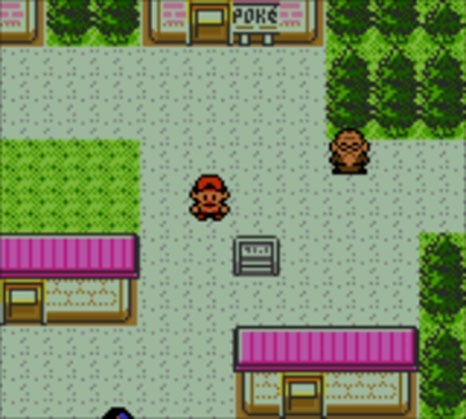
\includegraphics[width=6cm]{images/proposal/pokemon.png}}
    \legend{Source: \cite{pokemon:1999}}
    \label{fig:pokemon}
\end{figure}

\subsection{Map elements}

The tool chosen to develop our solution is the Unity game engine, which was released in 2005 and developed by Unity Technologies \cite{unity:2021}. Game engines are softwares that provide the core functionalities needed for a game to run, for example a rendering engine, a physics engine, a collision engine, etc. Figure \ref{fig:unity_print} shows a screenshot of this tool with some important elements that will be described on the next items of this section. The description of such elements have been adapted from \textcite{carvalho:2011}.

\begin{figure}[h]
    \caption{Screenshot of the Unity engine}
    \centerline{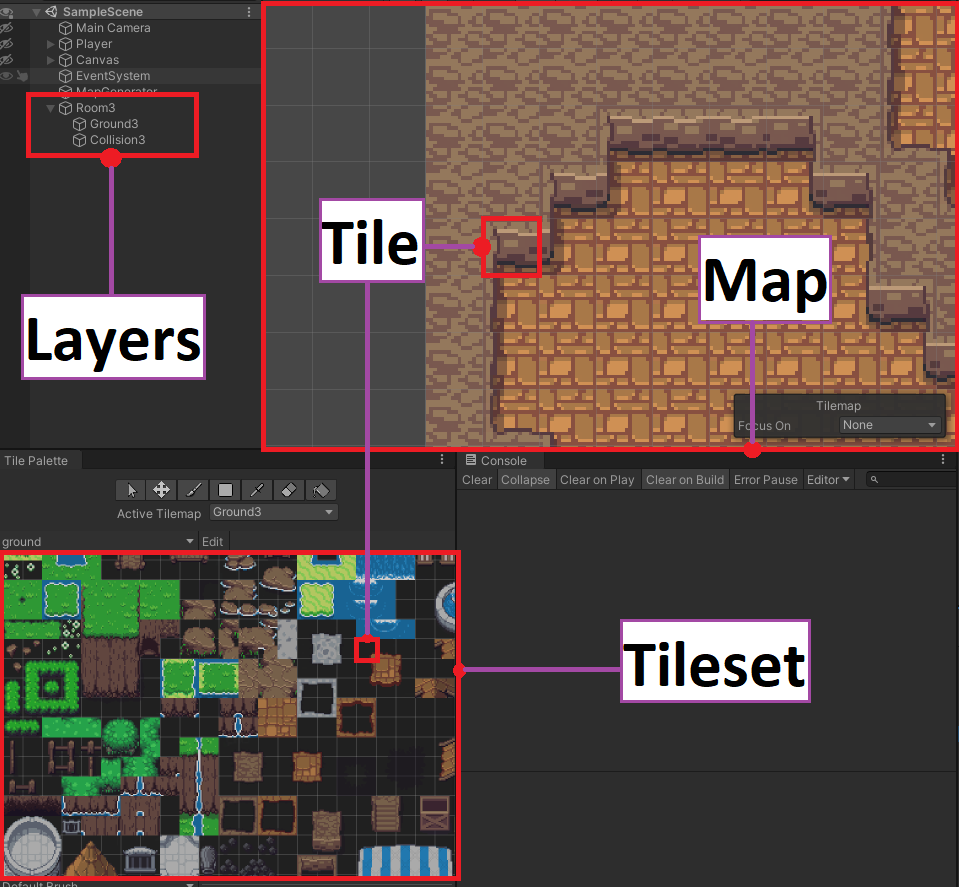
\includegraphics[width=11cm]{images/proposal/unity_print.png}}
    \legend{Source: Image provided by author}
    \label{fig:unity_print}
\end{figure}

\subsubsection{Map}
The map is represented here by a three-dimensional mesh of width \(w_{map}\) and height \(h_{map}\), with \{\(w_{map}, h_{map} \in \mathbb{N}|(w_{map}>0)\wedge(h_{map}>0)\)\}. Additionally, this mesh has a depth of \(l_{map}\) layers, with \{\(l_{map} \in \mathbb{N}|l_{map}\geq 1\)\}, in our specific case, \(l_{map} = 2\).

The map is composed by a number of \(w_{map} \times h_{map}\) cells, in our case, each cell has one or two tiles (which will be explained in a subsequent section) one per layer, creating what is called a tiled map. 

\subsubsection{Layers}
The layers are the different levels of the map where it's elements are distributed. In the scope of this work, there are two types of elements that will compose our maps, which are: ground and walls. The ground is the path where the player can walk on, while the walls are what define the structure of the cave maps. The player cannot walk on walls. In addition, these two elements are organized in two separate layers, here called ground layer and collision layer. The collision layer is named as such because, in order to avoid letting the player walk on the walls, a collider\footnote{In the Unity engine, the collider component is added to GameObjects where there's need to simulate physical collision.} component was added to this layer.

\subsubsection{Tiles}

A tile is the entity that occuppies the cells of the map mesh. Each tile is an image that represents some object to be inserted in the game, this image is of dimensions \((i*w_{cel})\times(j*h_{cel})\) with \(w_{cel}\) and \(h_{cel}\) representing, respectively, the width and height of a cell in the map, while \(i\) and \(j\) are constants where \{\(i, j \in \mathbb{N}|(1\leq i<w_{map})\wedge(1\leq j<h_{map})\)\}. In our specific case, \(w_{cel}=h_{cel}=16 {pixels}\) and all tiles used have \(i=j=1\). 
\subsubsection{Tileset}

A tileset is, as the name suggests, an image containing the set of tiles that will represent the game objects.

The Unity game engine divides any given tileset into a number of tiles that can be used by the developer to fill the map mesh and create an envinronment. The tileset used on this work is the "Zelda-like tileset", which was posted by \textcite{arm:2017} and is licensed in the public domain. Figure \ref{fig:tileset} shows this tileset, although only the tiles needed for walls and ground were used in this work, which will be shown in the next chapter.

\begin{figure}[h]
    \caption{Zelda-like tileset}
    \centerline{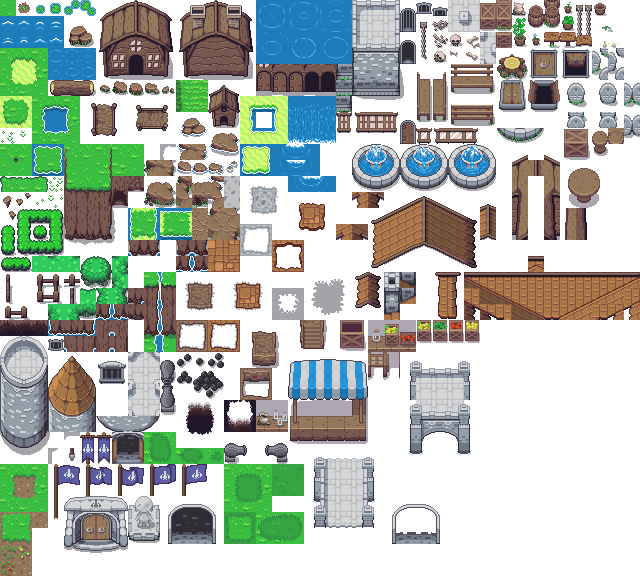
\includegraphics[width=10cm]{images/proposal/overworld.png}}
    \legend{Source: \cite{arm:2017}}
    \label{fig:tileset}
\end{figure}

\section{Cave patterns}

As will be discussed in the next section, one of the characteristics that make a good map is for it to have a natural look. Since we focused on cave-like maps, we researched for what would be understood as a natural cave representation in a 2D top-down view.

According to \textcite{audra:2011}, caves are formed by having different types of sources of water interacting with different kinds of soil. Figure \ref{fig:cave_patterns} show some of the most common cave patterns.

\begin{figure}[h]
    \caption{Common cave patterns}
    \centerline{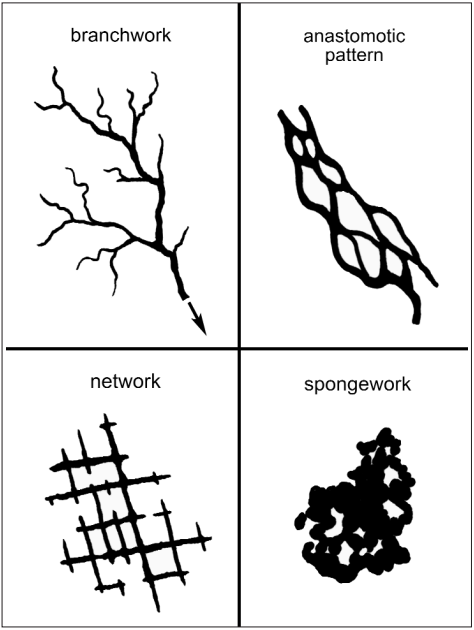
\includegraphics[width=6cm]{images/proposal/cave_patterns.png}}
    \legend{Source: \cite{audra:2011}}
    \label{fig:cave_patterns}
\end{figure}

It is outside of the scope of this work to give a larger description to each of the different cave patterns shown here, however it is important to note that this is an accurate representation of real-world caves and that they were used as a reference for the generated maps.

\section{What makes a good generated map}
\label{sec:goodmap}

At last, an important part of our proposal is to generate maps that have a set of qualities that make them be perceived as good or desirable maps by players.

During the bibliographic research for these criteria, most of the findings related not only to the map but to the entire game level entirely, for example in \textcite{preuss:2014} the placement of enemies and treasures are also taken into consideration.

However, there were some criteria found on such works that made reference only to the map itself. Here is a list of the qualities of a good generated map, according to our bibliographic research:

\begin{itemize}
\item The generated maps should have a natural look, they shouldn't look as if they were generated by an algorithm \cite{shaker:2016} \cite{adams:2002}.
\item Dungeon maps should have a point of entrance, a point of exit (which might be the same as the point of entrance), and a path between them \cite{shaker:2016}.
\item The Generated maps should look different from each other, to provide the player with an unique experience each time \cite{goncalves:2015} \cite{zapata:2014}.
\item The generated maps should encourage players to explore them \cite{ping:2020}.
\item Borders are necessary on the generated maps, in order to prevent players and monsters from escaping them \cite{torrado:2020}.
\end{itemize}

To evaluate if the generated maps have the qualities listed here, we created a survey based on the one found on \textcite{carvalho:2016}, which was used to evaluate players' motivation to explore game levels, developed based on the Instructional Materials Motivational Survey (IMMS), that uses the ARCS model by Keller \cite{keller:1987}, \cite{keller:1993}. Therefore, some of the elements for a good map that we will be evaluating are also adapted from the components of the ARCS model:

\begin{itemize}
    \item \textbf{Attention}:
    \begin{itemize}
        \item The design of the generated maps should be able to keep the player attention on the game.
        \item The generated maps' design should be attractive to the players.
    \end{itemize}
    \item \textbf{Relevance}:
    \begin{itemize}
        \item The player should want to play a game that includes the generated maps.
    \end{itemize}
    \item \textbf{Confidence}: 
    \begin{itemize}
        \item The generated maps should not appear to be too hard for the player.
        \item When looking at the map, the player should be able to comprehend it easily.
    \end{itemize}
    \item \textbf{Satisfaction}:
    \begin{itemize}
        \item The player should want to explore the map.
    \end{itemize}
\end{itemize}

More information about the survey will be given in Chapter \ref{chapter:survey}.
%  por fim falar da proposta: gerar um bom mapa em unity, o que é um bom mapa,